\documentclass[12pt]{article}

\usepackage[english]{babel}
\usepackage[utf8]{inputenc}
\usepackage{amsmath}
\usepackage{graphicx}
\usepackage[colorinlistoftodos]{todonotes}
\usepackage{listings}
\usepackage[font=small,labelfont=bf]{caption}
\usepackage{multirow}

\DeclareFixedFont{\ttb}{T1}{txtt}{bx}{n}{9} % for bold
\DeclareFixedFont{\ttm}{T1}{txtt}{m}{n}{9}  % for normal
% Defining colors
\usepackage{color}
\definecolor{deepblue}{rgb}{0,0,0.5}
\definecolor{deepred}{rgb}{0.6,0,0}
\definecolor{deepgreen}{rgb}{0,0.5,0}

\newcommand\pythonstyle{\lstset{
  language=Python,
  backgroundcolor=\color{white}, %%%%%%%
  basicstyle=\ttm,
  otherkeywords={self},            
  keywordstyle=\ttb\color{deepblue},
  emph={MyClass,__init__},          
  emphstyle=\ttb\color{deepred},    
  stringstyle=\color{deepgreen},
  commentstyle=\color{red},  %%%%%%%%
  frame=tb,                         
  showstringspaces=false            
}}


\lstnewenvironment{python}[1][]
{
\pythonstyle
\lstset{#1}
}
{}

\title{Numerical recipes project 2}

\author{Hakon Doelving s1575946}

\date{\today}

\begin{document}
\maketitle



\section{Introduction}
\label{sec:introduction}

The aim of this project is to use machine learning classification to determine weather types from ground based observations. Machine learning\newline classification is a way of teaching a computer to differentiate between certain given classes, in this case weather types, given certain features, in this case ground observations. For this to work there needs to be a correlation between the features and the classes.\newline This report will explore whether ground observations can be used to predict the weather type and how precise it can do it.

\section{Data}
\label{sec:data}
For this project a set of data was provided. The data consist of ground based weather observations made from 126 weather observation stations. The observations are made hourly during the period from 24th of October to 7th of November. This gives 45178 data points. Each data point consists of nine observational features, three locational features, one time feature and a weather type.
\begin{table}
\begin{center}
\begin{tabular}{| l | l | l | l | l | l |}
\hline
Data index & feature1 & feature2 & ... & feature n & weather type \\\hline
1 & temp1 & pressure1 & ... & elevation1 & clear \\
2 & temp2 & pressure2 & ... & elevation2 & cloudy \\
... & ... & ... & ... & ... & ... \\
n & temp n & pressure n & ... & elevation n & cloudy \\
\hline
\end{tabular}
\caption{\label{tab:widgets}Format of the data provided.}
\end{center}
\end{table}

\newpage

Some of the data provided had missing values. These values were all given the same value to keep the dimensions of the data points equal, and so they could be further modified if necessary.
\newline
The data was given in two files, one basic and one advanced. The basic file only had three categories for weather types whereas the advanced had eleven types.

\section{Methods}
One class and one script was provided for this project. The class, Weather, holds all the data from the ground based weather stations and enables \newline extraction and manipulation of that data. The script, FeatureExtract, \newline enabled the creation of the weather object, manipulation of it and the \newline possibility to choose which features were kept for further processing. Two methods were added to the Weather class to be able to extract the features selected in FeatureExtract from the weather object.
\subsection{Description of classifiers}
Four classifiers were used in this project; decision tree, artificial neural \newline network, nearest neighbours and random forest. All the classifiers are from the sklearn python package.
\subsubsection{Decision tree}
\begin{center}
\begin{tabular}{cc}
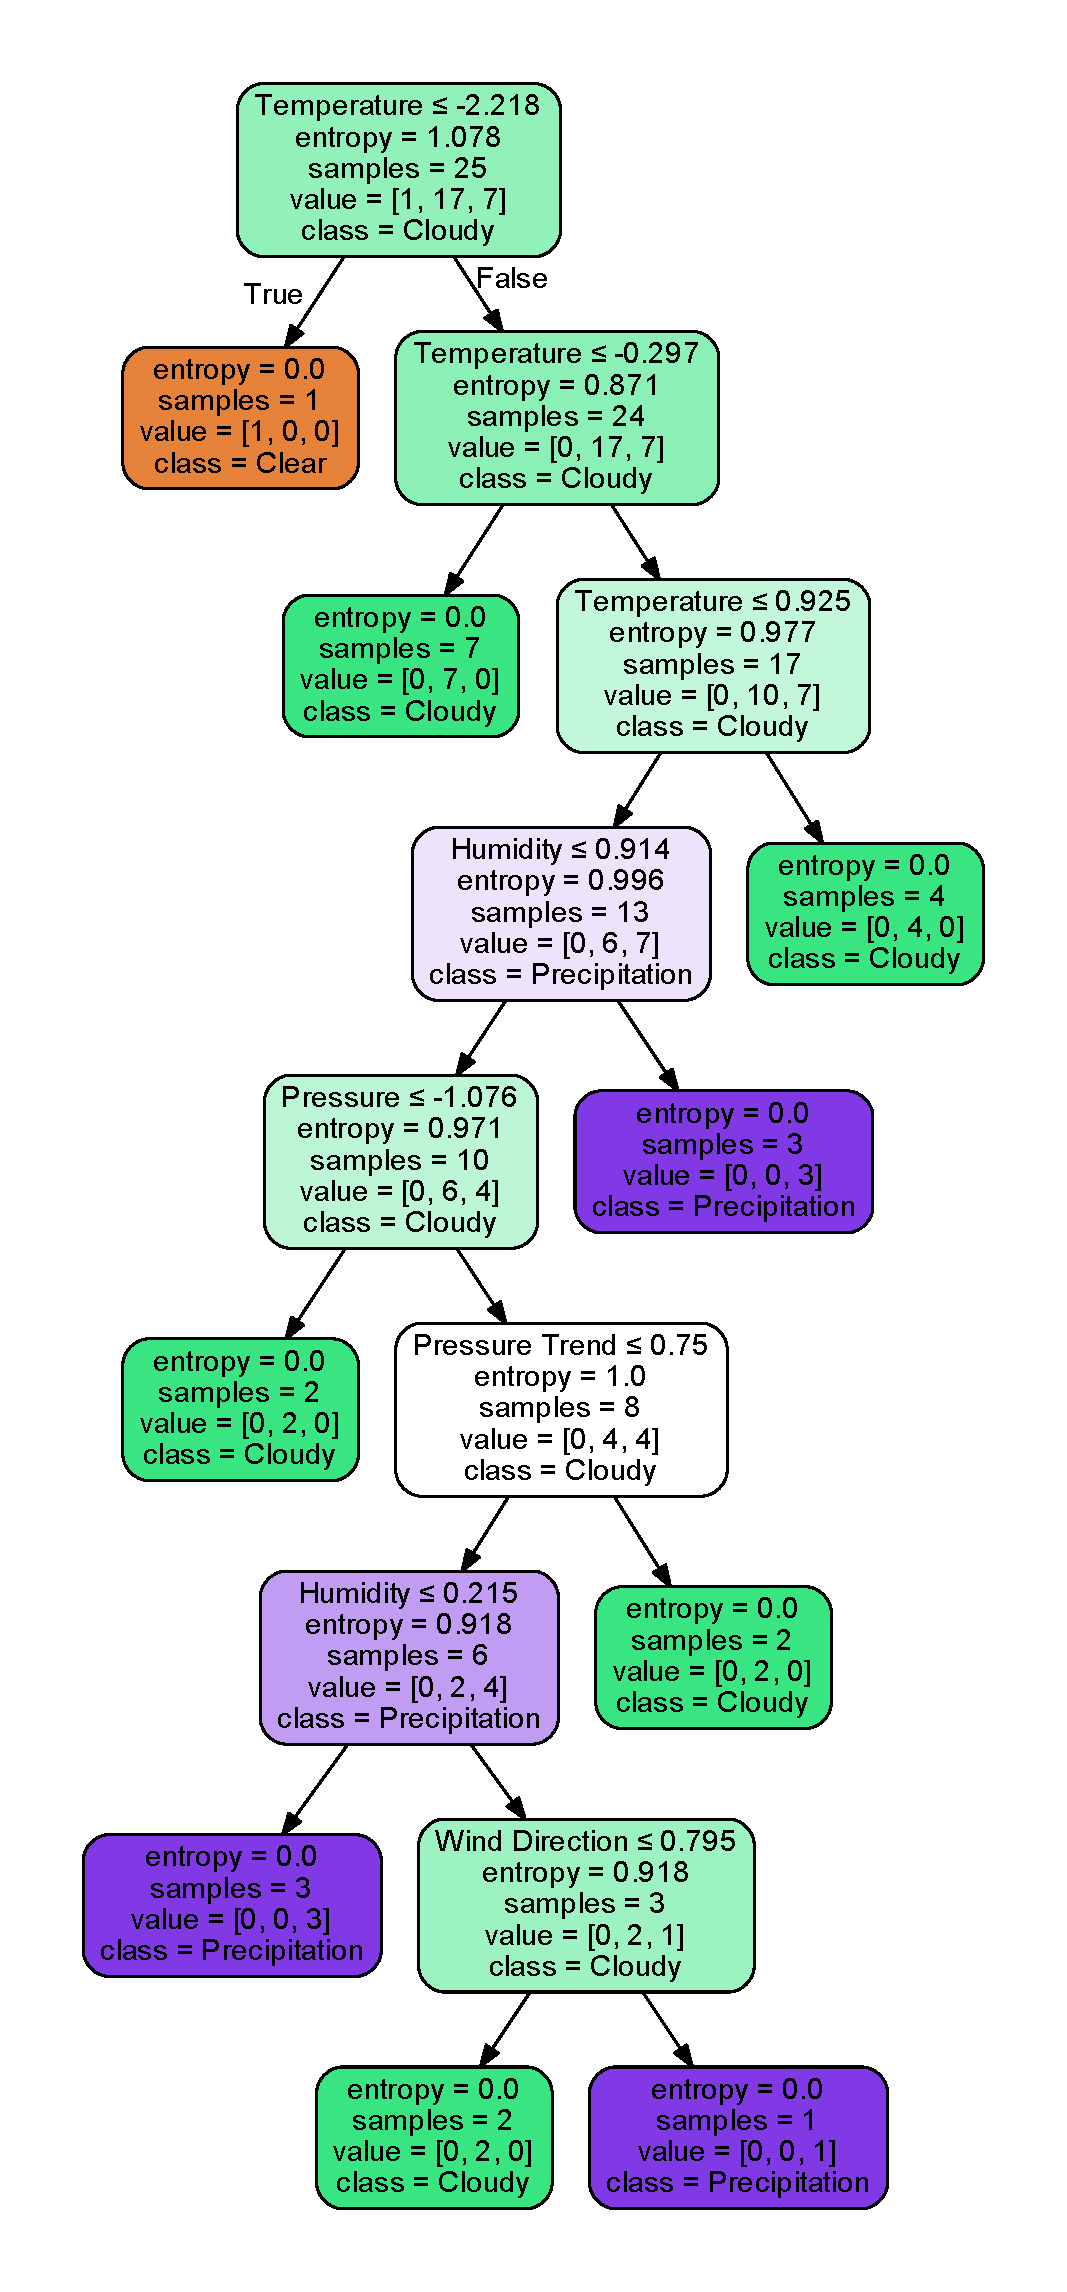
\includegraphics[scale = 0.2]{mini.pdf}
\end{tabular}
\captionof{figure}{Visual representation of decision tree generated from a small set of the provided data}
\end{center}

A decision tree classifier is a classifier that attempts to sort the data by learning simple true or false decision rules from the features. This is a so called white box model because it enables a user to look at the model and understand the decisions made. As can be seen in the figure, a decision tree has many boxes, or leaves. When the decision tree tries to predict a class from a set of features it propagates down the tree, from leaf to leaf, until it reaches a final leaf which defines it’s predicted class.

\subsubsection{Artificial neural network}

\begin{center}
\begin{tabular}{cc}
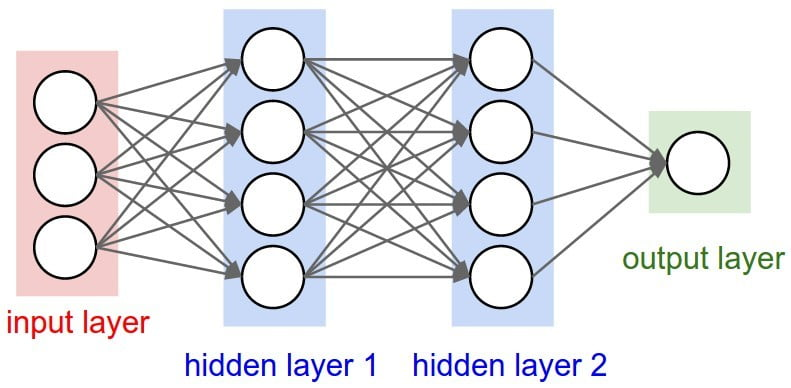
\includegraphics[scale = 0.2]{NN.jpg}
\end{tabular}
\captionof{figure}{Visual representation of an artificial neural network}
\end{center}
An artificial neural network classifier consists of an input layer, a set of hidden layers, each containing neurons and an output layer. The neural network learns to predict a class from a set of features by applying different weights to the features at each neuron. The input layer represents the features, where each neuron in the input layer is a feature. Each feature is then sent to all the neurons in the first hidden layer where they are applied a weight and summed up. Each hidden neuron has an activation function, meaning that the sum of the weighted inputs need to be a certain value for the neuron to activate and send a signal to the next layer. This propagates through the network untill the output layer receives an input which decides the output class. This is a black box model, meaning that it is hard to understand the decisions made by each neuron.

\subsubsection{Nearest neighbors}
\begin{center}
\begin{tabular}{cc}
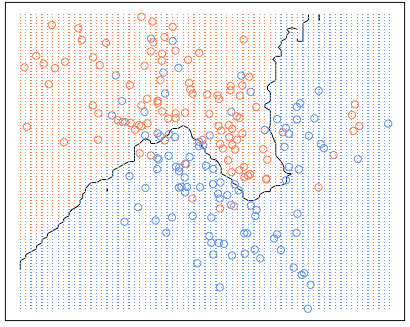
\includegraphics[scale = 0.5]{knn.png}
\end{tabular}
\captionof{figure}{Visual representation of nearest neighbours grouping}
\end{center}
A nearest neighbour classifier tries to predict the class by looking at the training data and picking out a predefined number samples that have \newline features that closely resembles that of the input. In a way, it is grouping the training data in n (features) space with boundaries that defines the class. A nearest neighbour classifier is therefore different from many other classifiers, it doesn’t try to make rules that decides what the output will be, but instead looks at the training data and compares it to the input features.

\subsubsection{Random forest}
\begin{center}
\begin{tabular}{cc}
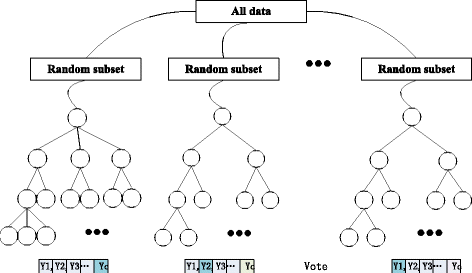
\includegraphics[scale = 0.5]{RF.png}
\end{tabular}
\captionof{figure}{Visual representation of a random forest}
\end{center}
A random forest classifier creates a set of decision trees, each with a different subset of features and weights. The splits are also decided by choosing the random best split instead of the best. This creates a forest of decision trees that will each produce an output class. The class that is finally returned is the one that the majority of the trees produce.


\subsection{Optimising}
A set of optimising techniques were used to try and increase precision and reduce overfitting.\newline
 Firstly, the data was standardised with the sklearn standardScaler. This means that the range of the data was changed so its mean became zero and its variance became one.\newline
 A grid-search was done on all the classifiers, meaning their initializing parameters were changed to find the ones that gave the best results for the given dataset.\newline
 A method for over sampling the data was implemented. This method looked at the class imbalance in the training data and made copies of the features and class of the underrepresented classes until all the classes were equally represented.\newline
A method for comparing the results from two or more classifiers trained and tested on the same data was implemented. This method would keep the testing results that were the same for all the classifiers. If it was not equal in all the classifiers it would keep the results that most of the classifiers agreed on, and if none of the classifiers agreed it would randomly pick the result from one of them, with all classifiers weighted equally.

\section{Results}
When comparing the classifiers there are two things that were looked at; precision and recall. The precision of a classifier is the ratio of true positives to false positives. I.e. what fraction of the predicted classes are actually that class. The recall of a classifier is the ratio of true positives to false negatives. I.e. what fraction of that class did the classifier predict correctly.



\begin{table}[!htbp]
\centering
\begin{tabular}{c | c | c | c | c |}
\cline{2-5}
 & Precision & Recall & F1-score & Support \\ \hline
\multicolumn{1}{ |c| }{Clear} & 0.48 & 0.50 & 0.49 & 4462 \\ \cline{1-1}
\multicolumn{1}{ |c| }{Cloudy} & 0.79 & 0.78 & 0.79 & 16057 \\ \cline{1-1}
\multicolumn{1}{ |c| }{Precipitation} & 0.37 & 0.38 & 0.38 & 2105 \\ \hline
\multicolumn{5}{ |c| }{}   \\ \hline
\multicolumn{1}{ |c| }{avg / total} & 0.69 & 0.69 & 0.69 & 22626 \\ \hline
\end{tabular}
\caption{\label{tab:widgets}Classification report of the decision tree without optimizing.}
\end{table}
From the classification report of the decision tree, using the features; Temperature, Visibility, Pressure, Pressure Trend, Humidity and Dew Point, and no optimising methods we got an average precision and recall of 0.69. There is also a big difference in the precision and recall between clear, cloudy and precipitation. This means that the classifier is overfitted to cloudy.
\newline
\newline
By standardising the data, performing a grid-search to find the best initializing parameters for the classifier, over-sampling the data, and using the features that, through trial and error, proved to give the best results (Temperature, Visibility, Pressure, Pressure Trend, Humidity, Dew Point, Wind direction, Latitude, Longitude) we see big improvements.

\begin{table}[!htbp]
\centering
\begin{tabular}{c | c | c | c | c |}
\cline{2-5}
 & Precision & Recall & F1-score & Support \\ \hline
\multicolumn{1}{ |c| }{Clear} & 0.58 & 0.56 & 0.57 & 4432 \\ \cline{1-1}
\multicolumn{1}{ |c| }{Cloudy} & 0.82 & 0.84 & 0.83 & 16088 \\ \cline{1-1}
\multicolumn{1}{ |c| }{Precipitation} & 0.52 & 0.52 & 0.38 & 2106 \\ \hline
\multicolumn{5}{ |c| }{}   \\ \hline
\multicolumn{1}{ |c| }{avg / total} & 0.75 & 0.75 & 0.75 & 22626 \\ \hline
\end{tabular}
\caption{\label{tab:widgets}Classification report of the decision tree with optimizing.}
\end{table}

\newpage

Both precision and recall improved for all classes, and the over fitting decreased some, but is still there. This can be seen easier by comparing the confusion matrices.

\begin{table}[!htbp]
%\begin{left}
\centering
\begin{tabular}{ c  c | c  c  c | l  l | c  c  c |}
\cline{3-10}
 &  & \multicolumn{3}{|c|}{Predicted class} & \multicolumn{2}{|c|}{ } & \multicolumn{3}{|c|}{Predicted class} \\\cline{3-5} \cline{8-10}
 &  & \multicolumn{1}{ |c| }{Clear} & \multicolumn{1}{ |c| }{Cloudy} & \multicolumn{1}{ |c| }{Precipitation} &  &  &\multicolumn{1}{ |c| }{Clear} & \multicolumn{1}{ |c| }{Cloudy} & \multicolumn{1}{ |c| }{Precipitation} \\\cline{1-5} \cline{8-10}
\multicolumn{1}{ |c| }{\multirow{3}{*}{True class}} & \multicolumn{1}{ |c| }{Clear} & 2217 & 2118 & 127 &   &  & 2497 & 1881 & 54 \\\cline{2-2}% \cline{8-10}
\multicolumn{1}{ |c| }{} & \multicolumn{1}{ |c| }{Cloudy} & 2258 & 12519 & 1282 &   &  & 1741 & 13437 & 910 \\\cline{2-2} %\cline{8-10}
\multicolumn{1}{ |c| }{} & \multicolumn{1}{ |c| }{Precipitation} & 129 & 1148 & 828 &   &  & 52 & 1002 & 1052 \\%\cline{2-10}
\hline
\end{tabular}
\caption{\label{tab:widgets}Left is confusion matrix of the decision tree without optimizing, right is with optimizing }
%\end{left}
\end{table}

To get better results it seems other classifiers need to be tested. Below is a graph of the results from them.

\begin{table}[!htbp]
%\begin{left}
\centering
\begin{tabular}{ |c  c  c  |}
\hline
\multicolumn{1}{ |c| }{Classifier} & \multicolumn{1}{ |c| }{Avg/total precision} & \multicolumn{1}{ |c| }{Avg/total recall} \\ \hline
\multicolumn{1}{ |c| }{Artificial neural network} & 0.78 & 0.79 \\ \cline{1-1}
\multicolumn{1}{ |c| }{Nearest neighbours} & 0.79 & 0.80 \\ \cline{1-1}
\multicolumn{1}{ |c| }{Random forest} & 0.82 & 0.83 \\ \cline{1-1}
\multicolumn{1}{ |c| }{Result comparison} & 0.81 & 0.81\\
\hline
\end{tabular}
\caption{\label{tab:widgets}Comparison of results from all classifiers. Full results can be seen in the appendix }
%\end{left}
\end{table}

From these results, the most interesting ones are the results from the random forest classifier and the results from the result comparison method applied to the three classifiers when the data is over sampled. \newline
The random forest classifier produces the results with the highest avg/total precision and recall, whereas the result comparison method produces the least overfitted results.


\newpage

\section{conclusion}



\newpage

%\begin{table}[!htbp]
%\begin{left}
%\centering
%\begin{tabular}{ c  c | c | c | c | }
%\cline{3-5}
 %&  & \multicolumn{3}{|c|}{Predicted class} \\\cline{3-5} 
% &  & Clear & Cloudy & Precipitation &  &  &Clear & Cloudy & Precipitation \\\cline{1-5} 
%\multicolumn{1}{ |c| }{\multirow{3}{*}{True class}} & Clear & 1000 & 0 & 0 &   &  & 2 & 0 & 0 \\\cline{2-5} 
%\multicolumn{1}{ |c| }{} & Cloudy & 0 & 40000 & 0 &   &  & 0 & 8 & 0 \\\cline{2-5} 
%\multicolumn{1}{ |c| }{} & Precipitation & 0 & 0 & 1000 &   &  & 0 & 0 & 4 \\\cline{2-5}

%\hline
%\end{tabular}
%\caption{\label{tab:widgets}Format of the data provided.}
%\end{left}
%\end{table}


\begin{table}[!htbp]
\centering
\begin{tabular}{c | c | c | c | c |}
\cline{2-5}
 & Precision & Recall & F1-score & Support \\ \hline
\multicolumn{1}{ |c| }{Clear} & 0.78 & 0.57 & 0.66 & 4414 \\ \cline{1-1}
\multicolumn{1}{ |c| }{Cloudy} & 0.78 & 0.57 & 0.66 & 4414 \\ \cline{1-1}
\multicolumn{1}{ |c| }{Precipitation} & 0.78 & 0.57 & 0.66 & 4414 \\ \hline
\multicolumn{5}{ |c| }{}   \\ \hline
\multicolumn{1}{ |c| }{avg / total} & 0.78 & 0.57 & 0.66 & 4414 \\ \hline
\end{tabular}
\caption{\label{tab:widgets}Format of the data provided.}

\end{table}


\begin{table}[!htbp]
%\begin{left}
\centering
\begin{tabular}{ c  c | c | c | c | l  l | c | c | c |}
\cline{3-10}
 &  & \multicolumn{3}{|c|}{Predicted class} & \multicolumn{2}{|c|}{ } & \multicolumn{3}{|c|}{Predicted class} \\\cline{3-5} \cline{8-10}
 &  & Clear & Cloudy & Precipitation &  &  &Clear & Cloudy & Precipitation \\\cline{1-5} \cline{8-10}
\multicolumn{1}{ |c| }{\multirow{3}{*}{True class}} & Clear & 1000 & 0 & 0 &   &  & 2 & 0 & 0 \\\cline{2-5} \cline{8-10}
\multicolumn{1}{ |c| }{} & Cloudy & 0 & 40000 & 0 &   &  & 0 & 8 & 0 \\\cline{2-5} \cline{8-10}
\multicolumn{1}{ |c| }{} & Precipitation & 0 & 0 & 1000 &   &  & 0 & 0 & 4 \\\cline{2-10}

\hline
\end{tabular}
\caption{\label{tab:widgets}Format of the data provided.}
%\end{left}
\end{table}



\newpage
\section{Apendix}

\subsection{Additional results}

\subsubsection{Artificial neural network}

\begin{table}[!htbp]
\centering
\begin{tabular}{c | c | c | c | c |}
\cline{2-5}
 & Precision & Recall & F1-score & Support \\ \hline
\multicolumn{1}{ |c| }{Clear} & 0.69 & 0.53 & 0.60 & 4443 \\ \cline{1-1}
\multicolumn{1}{ |c| }{Cloudy} & 0.82 & 0.90 & 0.86 & 16094 \\ \cline{1-1}
\multicolumn{1}{ |c| }{Precipitation} & 0.63 & 0.44 & 0.52 & 2089 \\ \hline
\multicolumn{5}{ |c| }{}   \\ \hline
\multicolumn{1}{ |c| }{avg / total} & 0.78 & 0.79 & 0.78 & 22626 \\ \hline
\end{tabular}
\caption{\label{tab:widgets}Classification report for Artificial neural network without over-sampling}
\end{table}


\begin{table}[!htbp]
\centering
\begin{tabular}{c | c | c | c | c |}
\cline{2-5}
 & Precision & Recall & F1-score & Support \\ \hline
\multicolumn{1}{ |c| }{Clear} & 0.53 & 0.71 & 0.60 & 4383 \\ \cline{1-1}
\multicolumn{1}{ |c| }{Cloudy} & 0.86 & 0.74 & 0.80 & 16162 \\ \cline{1-1}
\multicolumn{1}{ |c| }{Precipitation} & 0.44 & 0.60 & 0.51 & 2081 \\ \hline
\multicolumn{5}{ |c| }{}   \\ \hline
\multicolumn{1}{ |c| }{avg / total} & 0.76 & 0.72 & 0.73 & 22626 \\ \hline
\end{tabular}
\caption{\label{tab:widgets}Classification report for Artificial neural network with over-sampling}
\end{table}




\begin{table}[!htbp]
%\begin{left}
\centering
\begin{tabular}{ c  c | c | c | c | l  l | c | c | c |}
\cline{3-10}
 &  & \multicolumn{3}{|c|}{Predicted class} & \multicolumn{2}{|c|}{ } & \multicolumn{3}{|c|}{Predicted class} \\\cline{3-5} \cline{8-10}
 &  & Clear & Cloudy & Precipitation &  &  &Clear & Cloudy & Precipitation \\\cline{1-5} \cline{8-10}
\multicolumn{1}{ |c| }{\multirow{3}{*}{True class}} & Clear & 2377 & 2037 & 29 &   &  & 3101 & 1211 & 71 \\\cline{2-5} \cline{8-10}
\multicolumn{1}{ |c| }{} & Cloudy & 1031 & 14558 & 505 &   &  & 2712 & 11952 & 1498 \\\cline{2-5} \cline{8-10}
\multicolumn{1}{ |c| }{} & Precipitation & 14 & 1146 & 929 &   &  & 82 & 742 & 1257 \\\cline{2-10}

\hline
\end{tabular}
\caption{\label{tab:widgets}Left is confusion matrix of the Artificial neural network without over-sampling, right is with over-sampling .}
%\end{left}
\end{table}

\newpage

\subsubsection{Nearest neighbours}

\begin{table}[!htbp]
\centering
\begin{tabular}{c | c | c | c | c |}
\cline{2-5}
 & Precision & Recall & F1-score & Support \\ \hline
\multicolumn{1}{ |c| }{Clear} & 0.76 & 0.48 & 0.59 & 4443 \\ \cline{1-1}
\multicolumn{1}{ |c| }{Cloudy} & 0.81 & 0.94 & 0.87 & 16094 \\ \cline{1-1}
\multicolumn{1}{ |c| }{Precipitation} & 0.74 & 0.36 & 0.48 & 2089 \\ \hline
\multicolumn{5}{ |c| }{}   \\ \hline
\multicolumn{1}{ |c| }{avg / total} & 0.79 & 0.80 & 0.78 & 22626 \\ \hline
\end{tabular}
\caption{\label{tab:widgets}Classification report for nearest neighbours without over-sampling}
\end{table}


\begin{table}[!htbp]
\centering
\begin{tabular}{c | c | c | c | c |}
\cline{2-5}
 & Precision & Recall & F1-score & Support \\ \hline
\multicolumn{1}{ |c| }{Clear} & 0.51 & 0.83 & 0.63 & 4383 \\ \cline{1-1}
\multicolumn{1}{ |c| }{Cloudy} & 0.92 & 0.60 & 0.72 & 16162 \\ \cline{1-1}
\multicolumn{1}{ |c| }{Precipitation} & 0.35 & 0.82 & 0.49 & 2081 \\ \hline
\multicolumn{5}{ |c| }{}   \\ \hline
\multicolumn{1}{ |c| }{avg / total} & 0.79 & 0.66 & 0.69 & 22626 \\ \hline
\end{tabular}
\caption{\label{tab:widgets}Classification report for nearest neighbours with over-sampling}
\end{table}




\begin{table}[!htbp]
%\begin{left}
\centering
\begin{tabular}{ c  c | c | c | c | l  l | c | c | c |}
\cline{3-10}
 &  & \multicolumn{3}{|c|}{Predicted class} & \multicolumn{2}{|c|}{ } & \multicolumn{3}{|c|}{Predicted class} \\\cline{3-5} \cline{8-10}
 &  & Clear & Cloudy & Precipitation &  &  &Clear & Cloudy & Precipitation \\\cline{1-5} \cline{8-10}
\multicolumn{1}{ |c| }{\multirow{3}{*}{True class}} & Clear & 2153 & 2283 & 7 &   &  & 3645 & 607 & 131 \\\cline{2-5} \cline{8-10}
\multicolumn{1}{ |c| }{} & Cloudy & 681 & 15164 & 249 &   &  & 3443 & 9689 & 3030 \\\cline{2-5} \cline{8-10}
\multicolumn{1}{ |c| }{} & Precipitation & 6 & 1341 & 742 &   &  & 94 & 275 & 1712 \\\cline{2-10}

\hline
\end{tabular}
\caption{\label{tab:widgets}Left is confusion matrix of the nearest neighbours without over-sampling, right is with over-sampling .}
%\end{left}
\end{table}



\newpage

\subsubsection{Random forest}

\begin{table}[!htbp]
\centering
\begin{tabular}{c | c | c | c | c |}
\cline{2-5}
 & Precision & Recall & F1-score & Support \\ \hline
\multicolumn{1}{ |c| }{Clear} & 0.78 & 0.58 & 0.67 & 4335 \\ \cline{1-1}
\multicolumn{1}{ |c| }{Cloudy} & 0.84 & 0.94 & 0.89 & 16203 \\ \cline{1-1}
\multicolumn{1}{ |c| }{Precipitation} & 0.78 & 0.46 & 0.58 & 2088 \\ \hline
\multicolumn{5}{ |c| }{}   \\ \hline
\multicolumn{1}{ |c| }{avg / total} & 0.82 & 0.83 & 0.82 & 22626 \\ \hline
\end{tabular}
\caption{\label{tab:widgets}Classification report for Random forest without over-sampling}
\end{table}


\begin{table}[!htbp]
\centering
\begin{tabular}{c | c | c | c | c |}
\cline{2-5}
 & Precision & Recall & F1-score & Support \\ \hline
\multicolumn{1}{ |c| }{Clear} & 0.72 & 0.68 & 0.70 & 4383 \\ \cline{1-1}
\multicolumn{1}{ |c| }{Cloudy} & 0.86 & 0.90 & 0.88 & 16162 \\ \cline{1-1}
\multicolumn{1}{ |c| }{Precipitation} & 0.68 & 0.56 & 0.62 & 2081 \\ \hline
\multicolumn{5}{ |c| }{}   \\ \hline
\multicolumn{1}{ |c| }{avg / total} & 0.82 & 0.82 & 0.82 & 22626 \\ \hline
\end{tabular}
\caption{\label{tab:widgets}Classification report for Random forest with over-sampling}
\end{table}




\begin{table}[!htbp]
%\begin{left}
\centering
\begin{tabular}{ c  c | c | c | c | l  l | c | c | c |}
\cline{3-10}
 &  & \multicolumn{3}{|c|}{Predicted class} & \multicolumn{2}{|c|}{ } & \multicolumn{3}{|c|}{Predicted class} \\\cline{3-5} \cline{8-10}
 &  & Clear & Cloudy & Precipitation &  &  &Clear & Cloudy & Precipitation \\\cline{1-5} \cline{8-10}
\multicolumn{1}{ |c| }{\multirow{3}{*}{True class}} & Clear & 2531 & 1797 & 7 &   &  & 2977 & 1395 & 11 \\\cline{2-5} \cline{8-10}
\multicolumn{1}{ |c| }{} & Cloudy & 726 & 15207 & 270 &   &  & 1135 & 14488 & 539 \\\cline{2-5} \cline{8-10}
\multicolumn{1}{ |c| }{} & Precipitation & 7 & 1122 & 959 &   &  & 28 & 883 & 1170 \\\cline{2-10}

\hline
\end{tabular}
\caption{\label{tab:widgets}Left is confusion matrix of the Random forest without over-sampling, right is with over-sampling .}
%\end{left}
\end{table}

\newpage

\subsubsection{Result comparison}

\begin{table}[!htbp]
\centering
\begin{tabular}{c | c | c | c | c |}
\cline{2-5}
 & Precision & Recall & F1-score & Support \\ \hline
\multicolumn{1}{ |c| }{Clear} & 0.77 & 0.56 & 0.65 & 4335 \\ \cline{1-1}
\multicolumn{1}{ |c| }{Cloudy} & 0.83 & 0.94 & 0.88 & 16203 \\ \cline{1-1}
\multicolumn{1}{ |c| }{Precipitation} & 0.77 & 0.42 & 0.55 & 2088 \\ \hline
\multicolumn{5}{ |c| }{}   \\ \hline
\multicolumn{1}{ |c| }{avg / total} & 0.81 & 0.82 & 0.81 & 22626 \\ \hline
\end{tabular}
\caption{\label{tab:widgets}Classification report for Result comparison without over-sampling}
\end{table}


\begin{table}[!htbp]
\centering
\begin{tabular}{c | c | c | c | c |}
\cline{2-5}
 & Precision & Recall & F1-score & Support \\ \hline
\multicolumn{1}{ |c| }{Clear} & 0.60 & 0.76 & 0.67 & 4383 \\ \cline{1-1}
\multicolumn{1}{ |c| }{Cloudy} & 0.89 & 0.79 & 0.83 & 16162 \\ \cline{1-1}
\multicolumn{1}{ |c| }{Precipitation} & 0.51 & 0.68 & 0.59 & 2081 \\ \hline
\multicolumn{5}{ |c| }{}   \\ \hline
\multicolumn{1}{ |c| }{avg / total} & 0.80 & 0.77 & 0.78 & 22626 \\ \hline
\end{tabular}
\caption{\label{tab:widgets}Classification report for Result comparison with over-sampling}
\end{table}




\begin{table}[!htbp]
%\begin{left}
\centering
\begin{tabular}{ c  c | c | c | c | l  l | c | c | c |}
\cline{3-10}
 &  & \multicolumn{3}{|c|}{Predicted class} & \multicolumn{2}{|c|}{ } & \multicolumn{3}{|c|}{Predicted class} \\\cline{3-5} \cline{8-10}
 &  & Clear & Cloudy & Precipitation &  &  &Clear & Cloudy & Precipitation \\\cline{1-5} \cline{8-10}
\multicolumn{1}{ |c| }{\multirow{3}{*}{True class}} & Clear & 2448 & 1880 & 7 &   &  & 3334 & 996 & 53 \\\cline{2-5} \cline{8-10}
\multicolumn{1}{ |c| }{} & Cloudy & 734 & 15213 & 256 &   &  & 2191 & 12690 & 1281 \\\cline{2-5} \cline{8-10}
\multicolumn{1}{ |c| }{} & Precipitation & 6 & 1201 & 881 &   &  & 54 & 615 & 1412 \\\cline{2-10}

\hline
\end{tabular}
\caption{\label{tab:widgets}Left is confusion matrix of the Result comparison without over-sampling, right is with over-sampling .}
%\end{left}
\end{table}

\newpage
\subsection{code}
\subsubsection{weather.py addition}
\begin{python}

    def setSelectedFeatures(self,features):
        self.selectedFeatures = features
        print(self.selectedFeatures)

    def getSelectedFeatures(self):
        return self.selectedFeatures[:-1]

\end{python}

\subsubsection{FeatureExtract.py}

\begin{python}

## Step 1 - `Weather` class
#
# Begin by importing the Weather class.
# Weather data is accessed through an instantation of the provided `Weather` class.

from Weather import *

## Step 2 - Load Weather data
#
# Create a new object (e.g. `weather`) of type `Weather`.
#
# As part of the instantiation provide:
# - weatherFile: The filename (either basic.txt or advanced.txt)
# - fileSlice: The number of lines to read from the chosen input file (0 is all)
#
# Use the fileSlice to limit the sample size for early evaluation

weatherFile = 'data/basic.txt'
fileSlice = 0
weather = Weather(weatherFile, fileSlice)

## Step 3 - Inspect the Data
'''
print '#'*50
print '# Step 3: Inspect the Data'
print '#'*50
print '\n'

# print data
print 'Weather Data:'
print weather.data

# print number of entries
print 'Number of entries: %s' % (weather.getNrEntries())

# print target names
print 'Number of targets: %s' % (weather.getNrTargets())

print 'Target names: %s' % (weather.getTargetNames())

# print features
print 'Number of features: %s' % (weather.getNrFeatures())

print 'Feature names: %s' % (weather.getFeatures())

# uncomment below to print station data
# print 'Number of weather stations: %s' % (weather.getNrStations())
# print 'Stations (ID, Name, Latitude, Longitude)'
# print weather.getStationData('all')

# Edinburgh and Shap station details
print 'Station data for EDINBURGH/GOGARBANK: %s' % (weather.getStationData('EDINBURGH/GOGARBANK'))
print 'Station data for ID 3225: %s' % (weather.getStationData('3225'))

# get data from one feature
print 'Temperature data: %s' % (weather.getFeatureData('Temperature'))
'''
## Step 4 - Recovering Incomplete Data
#
# Some of the observation values have a value of `-99999`
# This is a default value I inserted to indicate that the feature data was either not collected
# at the time of the observation or had a null value.
#
# Any data points that contain null observations need to be corrected to avoid problems
# with subsequent filtering and modifications.
#
# In some cases null values can either be interpolated or set to a default value.
#
# The large majority of null data is from the `Gust` measurement.
# Here I assume than no observation is the same as a zero value

# zero any null gust measurements
newG = ['0' if g == '-99999' else g for g in weather.getFeatureData('Gust')]
weather.modify('Gust', newG)
newPt = ['F' if g == '-99999' else g for g in weather.getFeatureData('Pressure Trend')]
weather.modify('Pressure Trend', newPt)
#print weather.getFeatureData('Gust')

## Step 5 - Removing Incomplete Data

# After recovering any data ensure you run the `discard()` method to
# remove any data with remaining null observations.

weather.discard()

## Step 6 - Data Conversion

# Some of the features have observation values that will be difficult for a machine learning estimator
# to interpret correctly (e.g. Wind Direction).

# You should ensure that all the features selected for a machine learning classification have a numeric value.

# In example 1 the pressure trend is changed from Falling, Static, Rising to 0,1,2
# In example 2 the Wind Direction is changed to a 16 point index starting from direction NNE.

# **Important**: Due to the limitations with the `Weather` class ensure that any observation data
# remains type `string` (e.g store '1' **not** 1).
# The `export()` method will convert all the values from `string` to `float` just before the export.

# Example 1 - Enumerate Pressure Trend (-1 falling, 0 static, 1 rising)

# define types
pTType = ['F', 'S', 'R']

# generate new pressure trend values
newPT = [str(pTType.index(p) - 1) for p in weather.getFeatureData('Pressure Trend') ]

# modify dataset
weather.modify('Pressure Trend', newPT)

#print 'Pressure Trend: %s' % (weather.getFeatureData('Pressure Trend'))

# Example 2 - Enumerate Wind direction (use 16 point compass index)

# define types
compassRose = ['NNE', 'NE', 'ENE', 'E', 'ESE', 'SE', 'SSE', 'S', 'SSW', 'SW', 'WSW', 'W', 'WNW', 'NW', 'NNW', 'N']

# generate and modify Wind direction
weather.modify('Wind Direction', [compassRose.index(w) for w in weather.getFeatureData('Wind Direction')])

#print 'Wind Direction: %s' % (weather.getFeatureData('Wind Direction'))

## Step 7 - Data Extraction

# The `getObservations()` method will enable you to filter the available data by
# Station ID, date, time and a selected feature.

# This may be helpful if you want to build an additional input feature for classification based
# on contextual information

# The example below retrieves the temperature and dew point for Edinburgh for 24th October
'''
print '\n'
print '#'*50
print '# Step 7: Data Extraction'
print '#'*50
print '\n'

stationId = weather.getStationData('EDINBURGH/GOGARBANK')
features = ['Time since midnight', 'Temperature', 'Dew Point']

print 'Temperature and Dew Point measurements for Edinburgh 24th October'
print '(Time since midnight (min), Temperature, Dew Point)'
print weather.getObservations('3166', obsDate='2017-10-24', features=features)
'''
# This can then be combined with location data
# Here, the Pressure, Pressure Trend and Wind direction from the nearest weather station
# 100km NW of Edinburgh for 24th October is shown
# (uncomment section)

# stationId = weather.getStationData('EDINBURGH/GOGARBANK')
#
# # get nearest stations 100k NW of Edinburgh station within a 75km threshold
# nearestStations = weather.findStations([stationId[2], stationId[3]], ['100', '-45'], maxThreshold=75)
#
# print '\n'
# print 'Nearest stations 100km NW of EDINBURGH/GOGARBANK'
# for s in nearestStations:
#     print s
#
# # use nearest station (index 0 )
# nearStationId = nearestStations[0]
#
# # get observations from nearest station on 24/10
# obsDate='2017-10-24'
# print '\n'
# print 'Using station %s on %s' % (nearStationId[1], obsDate)
# features = ['Time since midnight', 'Pressure', 'Pressure Trend', 'Wind Direction']
# print '(Time since midnight (min), Pressure, Pressure Trend, Wind Direction)'
# print weather.getObservations(nearStationId[0], obsDate=obsDate, features=features)

## Step 8 - Add new features

# You may get better insights into underlying patterns in the observations
# by extacting the provided data to generate new features.
#
# An example using the wind direction is shown below.
# The direction *relative* to the North and to the West is generated and appended to the dataset.

# set relative direction (assume 16 points)
points = 16
north = [abs((points / 2) - int(w))%(points / 2) for w in weather.getFeatureData('Wind Direction')]
west = [abs((points / 2) - int(w) - (points / 4))%(points / 2) for w in weather.getFeatureData('Wind Direction')]

# append to dataset
weather.append('Wind Relative North', north)
weather.append('Wind Relative West', west)

## Step 9 - Select features

# To finish create an array of strings containing a subset of the features
# you feel will perform best in the classification. Call the select() method to filter the data

features = ['Temperature',\
 'Visibilty',\
  'Pressure',\
   'Pressure Trend',\
    'Humidity',\
     'Dew Point',\
      'Wind Direction',\
       'Latitude',\
        'Longitude',\
        #'Time since midnight',\
        ]
weather.setSelectedFeatures(features)

weather.select(features)

## Step 10 - Export data

# Run the `export()` method to write the data of your selected features to file as a `pickle` object.

# This will move the target data ('Weather Type') into a new variable (`target`).

# **Note**: It is assumed that the *Station ID*  and *Station Name* will not be used
# as features for classification and are automatically stripped. The `export()` method
# will also strip out incomplete data before exporting to file.

weather.export('data/mldata.p')
#weather.export('data/mldata1.p')
#weather.export('data/mldata2.p')

\end{python}

\subsubsection{MachineLearning.py}


\begin{python}

import matplotlib.pyplot as plt
import numpy as np
import graphviz
from sklearn.model_selection import GridSearchCV

## Step 1 - Import and Data loading

# Import the sklearn modules you intend to use as part of your Machine Learning analysis
# (e.g. classifiers, metrics, model selection)

import pickle
# ADD SKLEARN MODULES FOR YOUR CHOSEN CLASSIFICATION METHOD HERE
# e.g. to load the decision tree estimator use: from sklearn.tree import DecisionTreeClassifier
from sklearn.tree import DecisionTreeClassifier, export_graphviz
from sklearn.metrics import classification_report, confusion_matrix
from sklearn.model_selection import train_test_split
from sklearn.preprocessing import StandardScaler

# Load the weather data you created by FeatureExtraction.py
weather = pickle.load(open('data/mldata.p'))

# Confirm that the data has loaded correctly by inspecting the data attributes in the `weather` object.

# ADD PRINT STATEMENTS HERE (SEE FeatureExtract.py FOR EXAMPLES)
print(weather.data[0])
print(weather.target[0])
## Step 2 - Define the training and testing sample
#
# Divide the weather data into a suitable training and testing sample.
# Start with a 50/50 split but make this easily adaptable for futher fitting evaluation.
#
# *Examples*:
trainIn, testIn, trainOut, testOut = train_test_split(weather.data, weather.target, test_size = 0.5, train_size = 0.5)  #`](http://scikit-learn.org/stable/modules/generated/sklearn.model_selection.train_test_split.html)


#------------------------standardising features-------------------------------------

scaler = StandardScaler()
scaler.fit(trainIn)
trainIn = scaler.transform(trainIn)
testIn = scaler.transform(testIn)


#--------------------------------------------------------------------------------

'''uncomment to use
#-----------------------------------over-sampling----------------------------------------
one=0
zero=0
two=0
for i in range(len(trainOut)):
    if trainOut[i] == '1':
        one+=1
    if trainOut[i]=='0':
        zero+=1
    if trainOut[i]=='2':
        two+=1
#print(one)
#print(zero)
#print(two)
#print()

index = 0
while one>zero:
    if trainOut[index] == '0':
        trainIn=np.vstack((trainIn,trainIn[index]))
        trainOut = np.append(trainOut, ['0'])
        zero+=1
    index+=1
index = 0
while one>two:
    if trainOut[index] == '2':
        trainIn=np.vstack((trainIn,trainIn[index]))
        trainOut = np.append(trainOut, ['2'])
        two+=1
    index+=1

#print(one)
#print(zero)
#print(two)

#---------------------------------------------------------------------------
'''


'''uncomment to use
#-------------------------------Grid-search--------------------------------------------

tuned_parameters = [{'criterion':['gini','entropy'],\
                    'splitter':['best'],\
                    'min_samples_split': [2],\
                    'min_samples_leaf': [1],\
                    'random_state': [None],\
                    'class_weight': ['balanced'],\
                    'presort': [False],\
                    'max_depth':[ 9,10,11,12,25],\
                    'min_weight_fraction_leaf':[0],\
                    'max_leaf_nodes':[None]}]


scores = ['precision', 'recall']

for score in scores:
    print("# Tuning hyper-parameters for %s" % score)
    print()

    clf = GridSearchCV(DecisionTreeClassifier(), tuned_parameters, cv=5,
                       scoring='%s_macro' % score)
    clf.fit(trainIn, trainOut)

    print("Best parameters set found on development set:")
    print()
    print(clf.best_params_)
    print()
    print("Grid scores on development set:")
    print()
    means = clf.cv_results_['mean_test_score']
    stds = clf.cv_results_['std_test_score']
    for mean, std, params in zip(means, stds, clf.cv_results_['params']):
        print("%0.3f (+/-%0.03f) for %r"
              % (mean, std * 2, params))
    print()

    print("Detailed classification report:")
    print()
    print("The model is trained on the full development set.")
    print("The scores are computed on the full evaluation set.")
    print()
    y_true, y_pred = testOut, clf.predict(testIn)
    print(classification_report(y_true, y_pred))
    print()



#-----------------------------------------------------------------------
'''





# DEFINE TRAINING AND TESTING SAMPLES AND TARGETS HERE

## Step 3 - Define the classification method

# This can be any of the estimators provided by Sklearn.
# I suggest you start with a *white box* method
# to better understand the process before trying something more advanced.

# DEFINE CLASSIFIER HERE
# e.g for a Decision tree: clf = DecisionTreeClassifier()
clf = DecisionTreeClassifier(criterion = 'entropy',\
                            min_samples_split = 2,\
                            presort = False,\
                            max_depth = None,\
                            )


## Step 4 - Fit the training data

# Run the `fit` method of your chosen estimator using the training data (and corresponding targets) as input

# RUN FIT METHOD HERE
print(weather.getSelectedFeatures())
clf = clf.fit(trainIn,trainOut)

'''uncomment to use
#---------------Create in image of the decision tree-------------------

dot_data = export_graphviz(clf, out_file=None, feature_names=weather.getSelectedFeatures(), class_names=weather.getTargetNames(), filled=True, rounded=True, special_characters=True)
graph = graphviz.Source(dot_data)
graph.render("mini")

#------------------------------------------------------------------------
'''
## Step 5 - Define the expected and predicted datasets


thelist = clf.predict(testIn)




true = 0
false = 0
ones=0
zeros = 0
twos = 0
for i in range(0, len(thelist)):
    if thelist[i] == testOut[i]:
        true += 1
    else:
        false += 1
    if thelist[i]=='1':
        ones+=1
    if thelist[i]=='0':
        zeros+=1
    if thelist[i]=='2':
        twos+=1


print(clf.score(testIn,testOut))
print("number of true values: " + str(true))
print("number of false values: " + str(false))
print(classification_report(testOut, thelist, target_names = weather.getTargetNames()))
print(thelist)
print(testOut)
print("0's " + str(zeros))
print("1's " + str(ones))
print("2's " + str(twos))
print(confusion_matrix(testOut, thelist))
print(clf.feature_importances_)
# Define `expected` as your *test* target values (i.e. **not** your *training* target values)
# and run the `predict` method on your chosen estimator using your *test data*

# DEFINE EXPECTED AND PREDICTED VALUES HERE

## Step 6 - Prediction Evaluation

# Use the `sklearn.metrics` module to compare the results using the expected and predicted datasets.

# Examples:
# - [Sklearn Model Evaluation](http://scikit-learn.org/stable/modules/model_evaluation.html#)
# - [Handwritten Digits example](http://scikit-learn.org/stable/auto_examples/classification/plot_digits_classification.html#sphx-glr-auto-examples-classification-plot-digits-classification-py)

# RUN PREDICTION EVALUATION METHODS HERE



\end{python}

\subsubsection{Neural.py  (file for computing the other classifiers)}


\begin{python}

import matplotlib.pyplot as plt
import numpy as np
import graphviz
import pickle
from sklearn.metrics import classification_report, confusion_matrix
from sklearn.model_selection import train_test_split
from sklearn.neural_network import MLPClassifier
from sklearn.preprocessing import StandardScaler
from sklearn.model_selection import GridSearchCV
from sklearn.neighbors import KNeighborsClassifier
from sklearn.preprocessing import Normalizer
from sklearn.tree import DecisionTreeClassifier
from sklearn.ensemble import RandomForestClassifier


weather = pickle.load(open('data/mldata.p'))






trainIn, testIn, trainOut, testOut = train_test_split(weather.data, weather.target, test_size = 0.5, train_size = 0.5)

'''uncomment to use
#-----------------------------------over-sampling----------------------------------------
one=0
zero=0
two=0
for i in range(len(trainOut)):
    if trainOut[i] == '1':
        one+=1
    if trainOut[i]=='0':
        zero+=1
    if trainOut[i]=='2':
        two+=1

#print(one)
#print(zero)
#print(two)
#print()

add = 0
index = 0
while one>zero:
    if trainOut[index] == '0':
        trainIn=np.vstack((trainIn,trainIn[index]))
        trainOut = np.append(trainOut, ['0'])
        zero+=1
        add+=1
    index+=1
index = 0
add = 0
while one>two:
    if trainOut[index] == '2':
        trainIn=np.vstack((trainIn,trainIn[index]))
        trainOut = np.append(trainOut, ['2'])
        two+=1
        add+=1
    index+=1

#print(one)
#print(zero)
#print(two)

#---------------------------------------------------------------------------
'''

#--------------------------proscessing data-------------------------------
'''uncomment to use
#------normalize data------
scaler = Normalizer()
scaler.fit(trainIn)
trainIn = scaler.transform(trainIn)
testIn = scaler.transform(testIn)
#---------------------------
'''

#------standardize data---------
scaler = StandardScaler()
scaler.fit(trainIn)
trainIn = scaler.transform(trainIn)
testIn = scaler.transform(testIn)
#--------------------------------

#------------------------------------------------------------------------------


'''uncomment to use
#---------------------------------Grid-search-----------------------------------------
tuned_parameters = [{'solver':['adam'],\
 'activation':['tanh'],\
 'alpha':[1e-5],\
  'hidden_layer_sizes':[(5,2), (10,10), (10,10,10), (25,25), (25,25,25), (40,40,40), (60,60), (60,60,60)],\
   'random_state': [2],\
   'tol':[1e-10],\
   'max_iter':[500],\
   'warm_start':[True],\
   'epsilon':[1e-4] }]


scores = ['precision', 'recall']

for score in scores:
    print("# Tuning hyper-parameters for %s" % score)
    print()

    clf = GridSearchCV(MLPClassifier(), tuned_parameters, cv=5,
                       scoring='%s_macro' % score)
    clf.fit(trainIn, trainOut)

    print("Best parameters set found on development set:")
    print()
    print(clf.best_params_)
    print()
    print("Grid scores on development set:")
    print()
    means = clf.cv_results_['mean_test_score']
    stds = clf.cv_results_['std_test_score']
    for mean, std, params in zip(means, stds, clf.cv_results_['params']):
        print("%0.3f (+/-%0.03f) for %r"
              % (mean, std * 2, params))
    print()

    print("Detailed classification report:")
    print()
    print("The model is trained on the full development set.")
    print("The scores are computed on the full evaluation set.")
    print()
    y_true, y_pred = testOut, clf.predict(testIn)
    print(classification_report(y_true, y_pred))
    print()




#---------------------------------------------------------------------------
'''

clf = MLPClassifier(solver='adam',\
                    activation = 'tanh',\
                    alpha=1e-10,\
                    hidden_layer_sizes=(40,40,40),\
                     max_iter = 500,\
                      random_state = 2,\
                      tol = 1e-10,\
                      verbose = False,\
                       warm_start = True,\
                        epsilon= 1e-6,\
                        #beta_1 = 0.9,\
                        #beta_2 = 0.999,\
                        #early_stopping = False,\
                        )


clf1 = KNeighborsClassifier(n_neighbors=50,\
                            weights = 'distance')

clf2 =RandomForestClassifier(max_depth=None,\
                            random_state=None,\
                            n_estimators = 200,\
                            min_samples_split = 3,\
                            #bootstrap = True,\
                            #oob_score = False,\
                            n_jobs = 5,\
                            verbose = 0,\
                            warm_start = False,\
                            class_weight = 'balanced_subsample')

#clf = MLPClassifier(solver='adam', alpha=0.000001, random_state=1)



print( trainOut)

clf = clf.fit(trainIn, trainOut)
clf1 = clf1.fit(trainIn, trainOut)
clf2 = clf2.fit(trainIn, trainOut)

thelist = clf.predict(testIn)
thelist1 = clf1.predict(testIn)
thelist2 = clf2.predict(testIn)

print("-------------Neural-----------")
print(classification_report(testOut, thelist, target_names = weather.getTargetNames()))

print(confusion_matrix(testOut, thelist))

print("----------------neighbors-------------------------------")
print(classification_report(testOut, thelist1, target_names = weather.getTargetNames()))
print(confusion_matrix(testOut, thelist1))
#print(classification_report(thelist, thelist1, target_names = weather.getTargetNames()))
#print(confusion_matrix(thelist, thelist1))

print("----------------random forest--------------------------------")
print(classification_report(testOut, thelist2, target_names = weather.getTargetNames()))
print(confusion_matrix(testOut, thelist2))


'''uncomment to use
#------------------result optimisation with two-----------------------------------
newlist = np.zeros(len(thelist), dtype = str)

for i in range(len(thelist)):
    if thelist2[i]==thelist1[i]:
        if thelist2[i]=='1':
            newlist[i] = '1'
        if thelist2[i]=='0':
            newlist[i] = '0'
        if thelist2[i]=='2':
            newlist[i] = '2'

    else:
        if thelist2[i] == '1':
            newlist[i] = thelist1[i]
        elif thelist1[i] == '1':
            newlist[i] = thelist2[i]
        else:
            if np.random.random()>0.5:
                newlist[i] = thelist2[i]
            else:
                newlist[i] = thelist1[i]

newlist.astype(str)
print("-------------------optimized-----------------")
print(classification_report(testOut, newlist, target_names = weather.getTargetNames()))
print(confusion_matrix(testOut, newlist))

#-------------------------------------
'''
#------------------result optimisation with three-----------------------------------
newlist = np.zeros(len(thelist), dtype = str)



for i in range(len(thelist)):
    if thelist[i]==thelist1[i] and thelist[i]==thelist2[i]:
        if thelist[i]=='1':
            newlist[i] = '1'
        if thelist[i]=='0':
            newlist[i] = '0'
        if thelist[i]=='2':
            newlist[i] = '2'
    else:
        if thelist[i]==thelist1[i]:
            newlist[i]=thelist[i]
        elif thelist[i] == thelist2[i]:
            newlist[i] = thelist[i]
        elif thelist1[i] == thelist2[i]:
            newlist[i] = thelist1[i]
        else:
            randomnr = np.random.random()
            if randomnr>0.66:
                newlist[i] = thelist[i]
            elif randomnr>0.33 and randomnr<=0.66:
                newlist[i] = thelist1[i]
            else:
                newlist[i] = thelist2[i]

newlist.astype(str)
print("-------------------optimized-----------------")
print(classification_report(testOut, newlist, target_names = weather.getTargetNames()))
print(confusion_matrix(testOut, newlist))


#-------------------------------------




\end{python}


\end{document}